\documentclass[12pt, letterpaper]{article}
\usepackage{graphicx}

\title{Marine Heat waves}
\author{James Munroe}
\date{August 2, 2020}

\begin{document}

\maketitle

\section{Introduction}

In September 2019, a high temperature event in Fortune Bay resulted in the die-off salmon at an aquaculture site in Fortune Bay. The media reported this as significant event for the Newfoundland and Labrador \footnote{https://www.cbc.ca/news/canada/newfoundland-labrador/fortune-bay-cleanup-1.5305994} and the event and its clean up was the subject of public discussion. 
 
The ocean temperature near the surface (known as the sea surface temperature or SST) under goes daily and monthly variability superimposed on both a daily and annual cycle.  It important to understand how common a high temperature events are the ocean, how long they could last, and how significant the temperature anomaly is from the seasonal norms for a particular area.  While the specifics of the September 2019 die-off are not investigated here, we look at some ocean temperatures the same geographic region and describe the frequency and severity of abnormally warm periods.

\subsection{Dataset}

There are many ways to measure SST include from instruments deployed from boat, remote observations from satellites, and moored buoys.  In this report we will look at marine buoys are part of the Environment Canada Meteorological Service of Canada (MSC) buoy network.  This data is available for download from http://www.meds-sdmm.dfo-mpo.gc.ca/isdm-gdsi/waves-vagues/data-donnees/index-eng.asp as CSV files. The format of the CSV files is documented here http://www.meds-sdmm.dfo-mpo.gc.ca/isdm-gdsi/waves-vagues/formats-eng.html. In particular, depending on the model of the marine buoy, several data field are available as shown in Table~\ref{tbl:datafields}. Measuring sea surface temperature is not straightforward since there are many definition of precisely where the temperature is being measured.  For this report, we will focus on \texttt{SSTP} as the variable of interest.

\begin{table}[h]
\begin{tabular}{|l|l|}
\hline
Variable & Description and units                                                      \\ \hline
\texttt{WDIR }    & Direction from which the wind is blowing ($^\circ$ True)                          \\
\texttt{WSPD}     & Horizontal wind speed (m/s)                                                \\
\texttt{WSS\$}    & Horizontal scalar wind speed (m/s)                                         \\
\texttt{GSPD}    & Gust wind speed (m/s)                                                      \\
\texttt{ATMS}     & Atmospheric pressure at sea level (mbar)                                   \\
\texttt{DRYT}     & Dry bulb temperature ($^\circ$ C)                                                  \\
\texttt{SSTP}     & Sea surface temperature ($^\circ$ C)                                               \\
\texttt{SLEV}     & Observed sea level                                                         \\
\texttt{SST1}     & Average sea temperature from the non-synoptic part \\
  & of WRIPS buoy data ($^\circ$ C) \\
\texttt{HAT\$}    & Water temperature from high accuracy \\ & temperature sensor ($^\circ$ C)               \\ \hline
\end{tabular}
\caption{Variables in marine buoy data}
\label{tbl:datafields}
\end{table}

\subsection{Marine Heat Waves}

To quantify whether SST for a particular area is indeed abnormally warm, we will use the Marine Heatwave (MHW) definition of Hobday et al. (manuscript submitted to Progress in Oceanography).  An algorithm for detecting a MHW has been implemented in the Python package `marineHeatWave`.

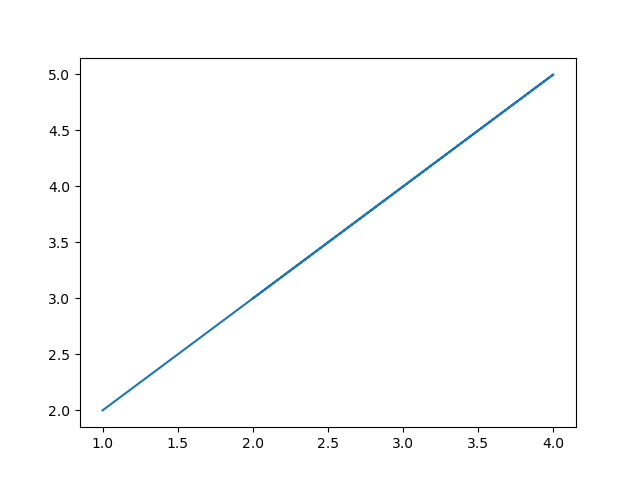
\includegraphics[width=0.9\textwidth]{myplot}

\end{document}
